\subsubsection{Iteration 3: Evaluation on Hovering Task}

This iteration focused on refining the PID controller and evaluating its performance in a hovering task.

\paragraph{Design}

To improve controller stability, the joystick update interval was adjusted to one update every 20 frames. In addition, the PID parameters were fine-tuned, as presented in \cref{table:pid_params}.

\begin{table}[h]
\centering
\caption{PID Controller Parameters} \label{table:pid_params}
\begin{tabular}{lccccc}
\hline
\textbf{Controller} & \textbf{Axis} & $K_p$ & $K_i$ & $K_d$ & Max Output \\
\hline
Position (Outer Loop) & X & 2.0 & 0.10 & 1.5 & 10 \\
Position (Outer Loop) & Y & 3.0 & 0.12 & 1.5 & 15 \\
Position (Outer Loop) & Z & 2.0 & 0.10 & 1.5 & 10 \\
\hline
Velocity (Inner Loop) & X & 1.0 & 0.05 & 0.3 & 8 \\
Velocity (Inner Loop) & Y & 1.5 & 0.10 & 0.5 & 12 \\
Velocity (Inner Loop) & Z & 1.0 & 0.05 & 0.3 & 8 \\
\hline
Yaw Control & Yaw & 3.0 & 0.00 & 1.0 & 5 \\
\hline
\end{tabular}
\end{table}

\paragraph{Enactment}

In the hovering task, the refined PID controller produced stable performance. As illustrated in \cref{fig:rl_hover}, both the PID controller (orange) and the RL agent (blue) were tasked with maintaining a constant altitude of 5 meters. Data were collected over a duration of 60 seconds. The results indicate that the PID controller maintained a stable hover, whereas the RL agent exhibited greater oscillation around the target height.

\begin{figure}[H]
    \caption{Hovering task results. The top plot shows throttle input, and the bottom plot shows drone altitude.}\label{fig:rl_hover}
    \centering
    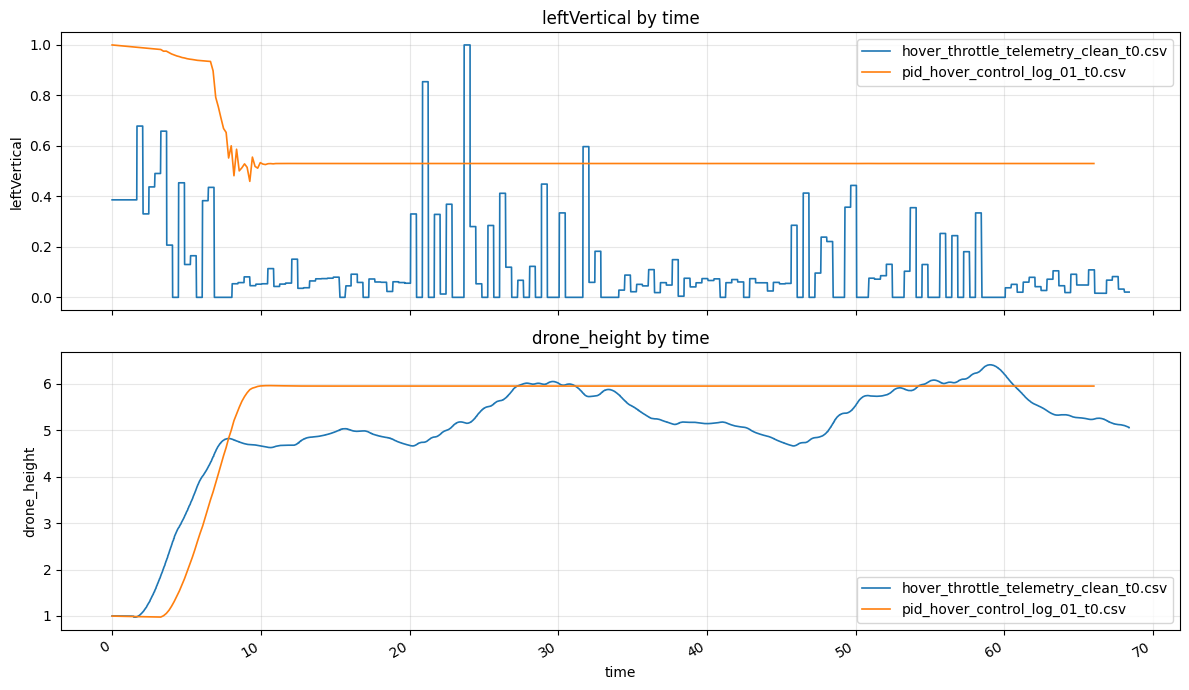
\includegraphics[width=0.8\linewidth]{img/result_hovering.png}
\end{figure}

\paragraph{Analysis}

After parameter tuning, the PID controller demonstrated stable and reliable altitude control in the hovering task. This level of performance was considered sufficient to proceed to the subsequent path-following evaluation.